\documentclass[]{article}
\usepackage[utf8]{inputenc}
\usepackage{polski}
\usepackage{listings}
\usepackage[usenames,dvipsnames]{xcolor}
\usepackage{geometry}
\usepackage{graphicx}
\usepackage{amsmath}
\usepackage{amssymb}
\usepackage{enumerate}
\graphicspath{ {./} }
\geometry{
	a4paper,
	left=25mm,
	right = 25mm,
	top=25mm,
}
%%\hyphenchar\font=-1

\title{
	Sprawozdanie \\
	\large 
	Obliczenia naukowe - lista 2}
\author{Kamil Król}
\date{244949}


\begin{document}
	
	\maketitle
	
	\section*{Zadanie 1}
	Celem tego zadania było powtórzenie zadania 5 z listy 1, ale ze zmianą danych i zobaczenie jak te zmiany wpłynęły na wynik. Modyfikacja danych polegała na usunięciu ostatniej 9 z x4 i ostatniej 7 z x5. \newline
	Dane początkowe:\newline
	\mbox{$x_1$ = [2.718281828, -3.141592654, 1.414213562, 0.5772156649, 0.3010299957]}\newline
	\mbox{$y_1$ = [1486.2497, 878366.9879, -22.37492, 4773714.647, 0.000185049].}\newline
	Dane po modyfikacji:\newline
	\mbox{$x_2$ = [2.718281828, -3.141592654, 1.414213562, 0.577215664, 0.301029995]}\newline
	\mbox{$y_2$ = [1486.2497, 878366.9879, -22.37492, 4773714.647, 0.000185049].}\newline
	Poniżej wyniki dla obu zestawów.
	
	\begin{table}[h!]
		\centering
		\label{tab:table1}
		\begin{tabular}{|c|c|c|c|}
			\multicolumn{4}{c}{Dla Float64 dla danych $x_1$ i $y_1$}\\ \hline
			alogrytm & obliczona wartość & błąd bezwzględny & błąd względny\\
			\hline
			Forward & 1.0251881368296672e-10 & 1.1258452438296672e-10 & 11.184955313981627 \\ \hline
			Backward & -1.5643308870494366e-10 & 1.4636737800494365e-10 & 14.541186645165915 \\ \hline
			Descending & 0.0 & 1.00657107e-11 & 1.0 \\ \hline
			Ascending & 0.0 & 1.00657107e-11 & 1.0 \\ \hline
		\end{tabular}
	\end{table}

\begin{table}[h!]
	\centering
	\label{tab:table1}
	\begin{tabular}{|c|c|c|c|}
		\multicolumn{4}{c}{Dla Float64 dla danych $x_2$ i $y_2$}\\
		\hline
		alogrytm & obliczona wartość & błąd bezwzględny & błąd względny\\
		\hline
		Forward & -0.004296342739891585 & 0.004296342729825875 & 4.2682954615672344e8 \\ \hline
		Backward & -0.004296342998713953 & 0.004296342988648243 & 4.2682957186999655e8 \\ \hline
		Descending & -0.004296342842280865 & 0.004296342832215154 & 4.268295563288099e8 \\ \hline
		Ascending & -0.004296342842280865 & 0.004296342832215154 & 4.268295563288099e8 \\ \hline
	\end{tabular}
\end{table}


\begin{table}[h!]
	\centering
	\label{tab:table1}
	\begin{tabular}{|c|c|c|c|}
		\multicolumn{4}{c}{Dla Float32 dla danych $x_1$ i $y_1$}\\
		\hline
		alogrytm & obliczona wartość & błąd bezwzględny & błąd względny\\
		\hline
		Forward & -0.4999443 & 0.49994429944939167 & 4.9668057661282845e10 \\ \hline
		Backward & -0.4543457 & 0.4543457031149343 & 4.51379655800096e10 \\ \hline
		Descending & -0.5 & 0.4999999999899343 & 4.967359135306107e10 \\ \hline
		Ascending & -0.5 & 0.4999999999899343 & 4.967359135306107e10 \\ \hline
	\end{tabular}
\end{table}

\begin{table}[h!]
	\centering
	\label{tab:table1}
	\begin{tabular}{|c|c|c|c|}
		\multicolumn{4}{c}{Dla Float32 dla danych $x_2$ i $y_2$}\\
		\hline
		alogrytm & obliczona wartość & błąd bezwzględny & błąd względny\\
		\hline
		Forward & -0.4999443 & 0.49994429944939167 & 4.9668057661282845e10 \\ \hline
		Backward & -0.4543457 & 0.4543457031149343 & 4.51379655800096e10 \\ \hline
		Descending & -0.5 & 0.4999999999899343 & 4.967359135306107e10 \\ \hline
		Ascending & -0.5 & 0.4999999999899343 & 4.967359135306107e10 \\ \hline
	\end{tabular}
\end{table}

Pierwszą obserwacją jest fakt, że wyniki dla typu Float32 są takie same dla obu zestawów testowych. Drugą obserwacją jest to, że dla typu Float64 niewielkie zmiany w danych wejściowych spowodowały duże różnice w wynikach. Wnioskiem z zadania jest to, że obliczanie iloczynku skalarnego jest zadaniem źle uwarunkowanym.


	
	
	\section*{Zadanie 2}
	
	Celem zadania było narysowanie wykresu funkcji $f(x) = e^{x}\cdot ln(1+e^{-x})$ w dwóch dowolnych programach do wizualizacji. Ponadto należało obliczyć granicę funkcji \(\lim\limits_{x \to \infty}f(x)\) i porównać wynik z otrzymanymi wykresami. Zacząłem od obliczenia granicy: \(\lim\limits_{x \to \infty}f(x).\)
\begin{equation}
\begin{aligned}
\mathop {\lim }\limits_{x \to \infty} f(x) &= \mathop {\lim }\limits_{x \to \infty} e^x \ln(1 + e^{-x}) = \mathop {\lim }\limits_{x \to \infty} \dfrac{\ln(1 + e^{-x})}{e^{-x}} = \left[\dfrac{0}{0}\right] \stackrel{H}{=} \mathop {\lim }\limits_{x \to \infty} \dfrac{(\ln(1 + e^{-x}))'}{(e^{-x})'} = \\ 
&= \mathop {\lim }\limits_{x \to \infty} \dfrac{\frac{1}{1 + e^{-x}}\cdot -e^{-x}}{-e^{-x}} = \mathop {\lim }\limits_{x \to \infty} \dfrac{1}{1 + e^{-x}} = 1. \nonumber
\end{aligned}
\end{equation}
	
	 Poniżej wykresy z dwóch programów do wizualizacji.
	
	
	\begin{figure}[!htbp]
		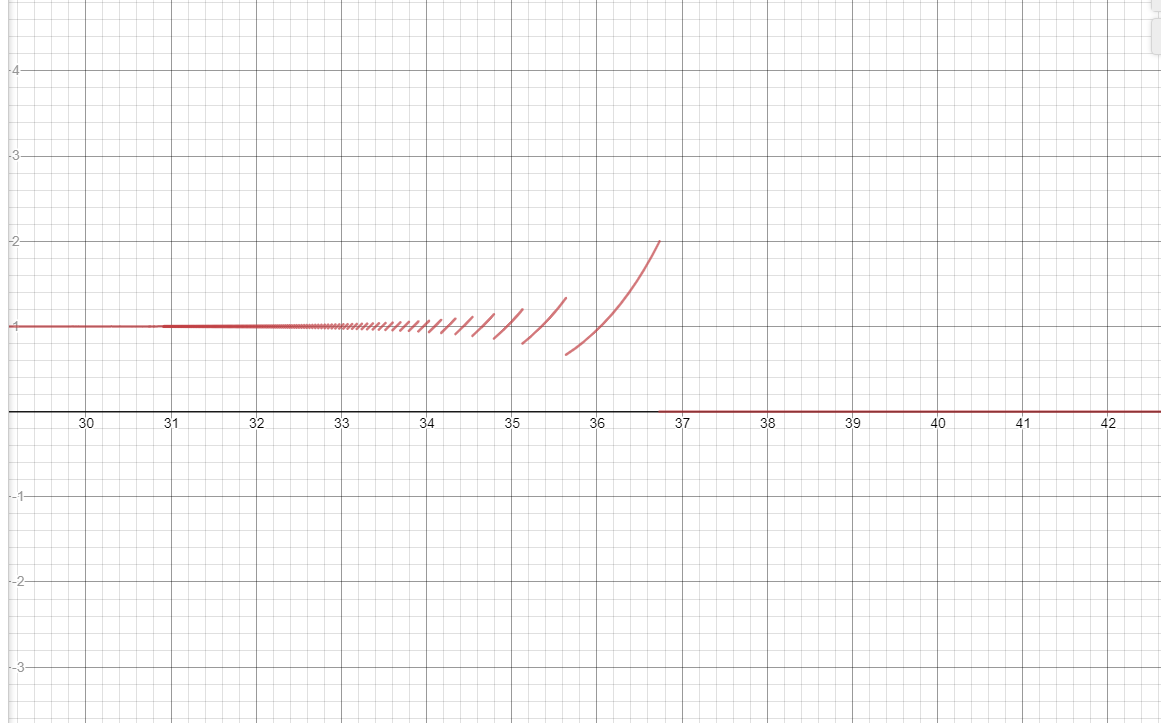
\includegraphics[scale=0.9]{task2_plot_desmos_broken}
		\centering
		\caption{Wykres funkcji f(x) narysowany w programie desmos}
	\end{figure}
	\clearpage
	\begin{figure}[!htbp]
		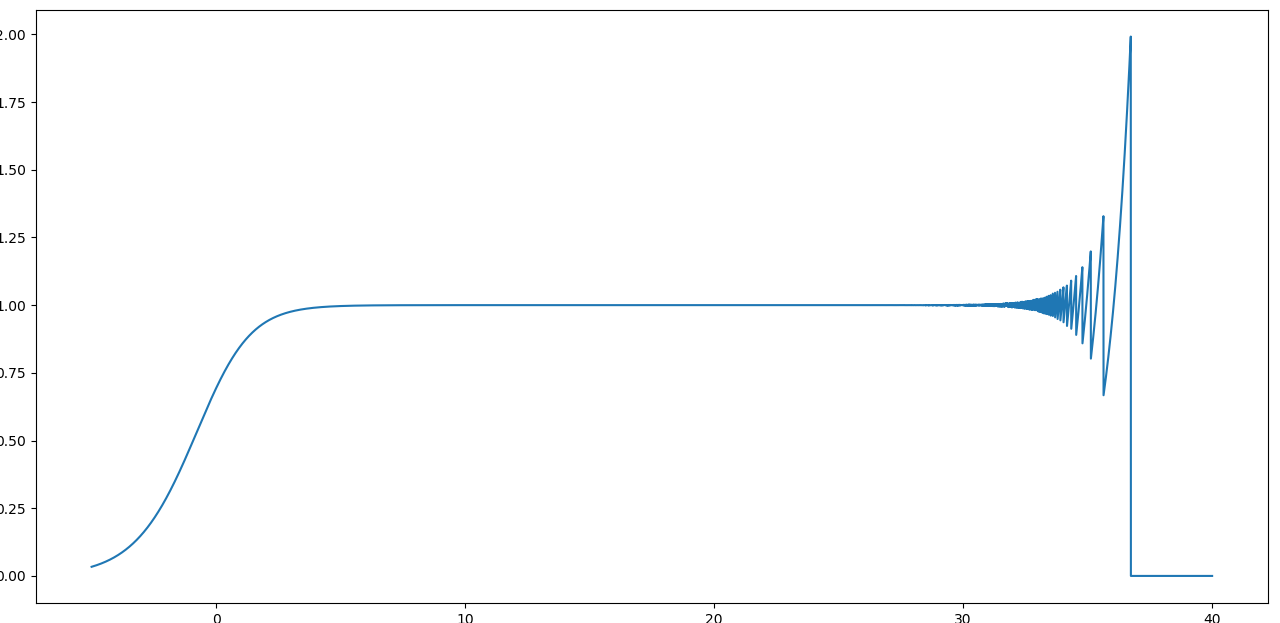
\includegraphics[scale=0.5]{task2_plot_pyplot}
		\centering
		\caption{Wykres funkcji f(x) narysowany w programie pyplot}
	\end{figure}

	Na wykresach można zaobserwować ze dla x pomiędzy 30, a 40 funkcja zaczyna się zachowywać w nieoczekiwany sposób. Widać też, że dla dwóch programów zachowanie jest różne. Ponadto żaden z wykresów nie pokazuje właściwego przebiegu funkcji, ponieważ jej granicą przy x zmierzającym do nieskończoności jest 1, a nie jak sugerują wykresy wartość 0. Ostatnią rzeczą do zrobienia w tym zadaniu jest wyjaśnienie tego zjawiska. W tym celu przyjrzyjmy się dokładniej funkcji  $f(x) = e^{x}\cdot ln(1+e^{-x})$. Ze wzoru widać, że im większy argument x weźmiemy tym mamy do czynienia z mnożeniem coraz większej liczby z coraz mniejszą. Inna rzecz to \textit{to co dzieje się pod logarytmem}.
	Jest tam dodawanie liczby 1 do bardzo małej liczby (w przypadku odpowiednio dużego x). Jeżeli czynnik $e^{-x}$ jest odpowiednio mały to następuje zjawisko pochłonięcia tej wartości i otrzymujemy wartość 1.0. Zauważmy, że $e^{-37} < 2^{-53} < eps()$ oraz $ln(1) = 0$. Daje to w rezultacie mnożenie $e^{-x}\cdot ln(1)=e^{-x}\cdot0 = 0$, a następnie błędny wykres. Wnioskiem z zadania jest to, że bardzo małe zmiany w danych spowodowały duże różnice w wyniku. Zatem jest to przykład zadania, które jest źle uwarunkowane.
	
	\clearpage

	\section*{Zadanie 3} 
	
	Celem zadania jest wykonanie eksperymentów opisanych w treści zadania dotyczących rozwiązywania równania $\mathbf{Ax = b}$. Gdzie $\mathbf{A} \in \mathbb{R}^{n\times n}$,  $\mathbf{b} \in \mathbb{R}^n$.
	Macierz A zadana jest jako:
	\begin{enumerate}[a)]
		\item macierz Hilberta $\mathbf{H}_n$ stopnia $n$,
		\item macierz losowa $\mathbf{R}_n^c$ stopnia $n$ o danym wskaźniku uwarunkowania $c$.
	\end{enumerate}
	Wektor $\mathbf{b}$ dany jest jako $\mathbf{b = Ax}$, gdzie $\mathbf{x} = (1, \dots, 1)^{T}$. Dzięki temu znamy dokładne rozwiązanie dla A i b. Układ równań $\mathbf{Ax} = \mathbf{b}$ należało rozwiązać za pomocą dwóch algorytmów:
	\begin{enumerate}[a)]
		\item metodą eliminacji Gaussa: $\mathbf{x} = \mathbf{A} \backslash \mathbf{b}$,
		\item metodą macierzy odwrotnej: $\mathbf{x} = \mathbf{A}^{-1}\mathbf{b}$.
	\end{enumerate}
	Poniżej znajdują się wyniki eksperymentów.
	
	\begin{table}[h!]
		\centering
		\label{tab:table1}
		\begin{tabular}{|c|c|c|c|c|c|}
			\hline
			\multicolumn{5}{|c|}{Wyniki dla macierzy Hilberta} \\
			\hline
			rozmiar & rank & cond & błąd względny dla gaussa & błąd względny dla odwrotności \\ 
			\hline
			2 x 2 & 2 & 19.28147006790397 & 5.661048867003676e-16 & 1.4043333874306803e-15 \\ \hline
			3 x 3 & 3 & 524.0567775860644 & 8.022593772267726e-15 & 0.0 \\ \hline
			4 x 4 & 4 & 15513.73873892924 & 4.137409622430382e-14 & 0.0 \\ \hline
			5 x 5 & 5 & 476607.25024259434 & 1.6828426299227195e-12 & 3.3544360584359632e-12 \\ \hline
			6 x 6 & 6 & 1.4951058642254665e7 & 2.618913302311624e-10 & 2.0163759404347654e-10 \\ \hline
			7 x 7 & 7 & 4.75367356583129e8 & 1.2606867224171548e-8 & 4.713280397232037e-9 \\ \hline
			8 x 8 & 8 & 1.5257575538060041e10 & 6.124089555723088e-8 & 3.07748390309622e-7 \\ \hline
			9 x 9 & 9 & 4.931537564468762e11 & 3.8751634185032475e-6 & 4.541268303176643e-6 \\ \hline
			10 x 10 & 10 & 1.6024416992541715e13 & 8.67039023709691e-5 & 0.0002501493411824886 \\ \hline
			11 x 11 & 10 & 5.222677939280335e14 & 0.00015827808158590435 & 0.007618304284315809 \\ \hline
			12 x 12 & 11 & 1.7514731907091464e16 & 0.13396208372085344 & 0.258994120804705 \\ \hline
			13 x 13 & 11 & 3.344143497338461e18 & 0.11039701117868264 & 5.331275639426837 \\ \hline
			14 x 14 & 11 & 6.200786263161444e17 & 1.4554087127659643 & 8.71499275104814 \\ \hline
			15 x 15 & 12 & 3.674392953467974e17 & 4.696668350857427 & 7.344641453111494 \\ \hline
		\end{tabular}
	\end{table}

	\begin{table}[h!]
		\centering
		\label{tab:table1}
		\begin{tabular}{|c|c|c|c|c|c|}
			\hline
			\multicolumn{5}{|c|}{Wyniki dla macierzy losowej} \\
			\hline
			rozmiar & rank & cond & błąd względny dla gaussa & błąd względny dla odwrotności \\ 
			\hline
			5 x 5 & 5 & 1.0 & 2.2752801345137457e-16 & 1.1102230246251565e-16 \\ \hline
			5 x 5 & 5 & 10.0 & 3.8459253727671276e-16 & 2.482534153247273e-16 \\ \hline
			5 x 5 & 5 & 1000.0 & 9.239830705567284e-15 & 8.255760547102576e-15 \\ \hline
			5 x 5 & 5 & 1.0e7 & 2.677573588098912e-10 & 1.4018261081995785e-10 \\ \hline
			5 x 5 & 5 & 1.0e12 & 1.1188918281429124e-5 & 1.5777474445400015e-5 \\ \hline
			5 x 5 & 4 & 1.0e16 & 0.5599366084107262 & 0.570943572080464 \\ \hline
			10 x 10 & 10 & 1.0 & 3.6821932062951477e-16 & 2.1925147983971603e-16 \\ \hline
			10 x 10 & 10 & 10.0 & 2.6272671962866383e-16 & 3.6316343785083587e-16 \\ \hline
			10 x 10 & 10 & 1000.0 & 3.155065537791195e-15 & 4.089480552672362e-15 \\ \hline
			10 x 10 & 10 & 1.0e7 & 1.1578006231204614e-10 & 1.1234229352336132e-10 \\ \hline
			10 x 10 & 10 & 1.0e12 & 3.319411920794968e-6 & 6.607249479556569e-6 \\ \hline
			10 x 10 & 9 & 1.0e16 & 0.09597742941854902 & 0.08790571295190734 \\ \hline
			20 x 20 & 20 & 1.0 & 5.7635440208947e-16 & 3.9720546451956367e-16 \\ \hline
			20 x 20 & 20 & 10.0 & 4.256659361141682e-16 & 4.902612130890297e-16 \\ \hline
			20 x 20 & 20 & 1000.0 & 4.556042017608055e-15 & 7.992372100964234e-15 \\ \hline
			20 x 20 & 20 & 1.0e7 & 1.197252918540844e-10 & 3.1220980667373144e-11 \\ \hline
			20 x 20 & 20 & 1.0e12 & 4.354484314307619e-5 & 4.162108310059814e-5 \\ \hline
			20 x 20 & 19 & 1.0e16 & 0.0675922370477866 & 0.09120905545435168 \\ \hline
		\end{tabular}
	\end{table}

	Patrząc na tabelę pierwszą - wyniki dla macierzy Hilberta, można zauważyć zależność błędu względnego od wskaźnika uwarunkowania. Im większy jest wskaźnik uwarunkowania tym większy jest błąd. Macierz Hilberta jest przykładem macierzy, która jest bardzo źle uwarunkowana. Widać też, że metoda eliminacji Gaussa okazała się w tym przypadku dokładniejsza dla $n>7$. \newline
	Patrząc na tabelę drugą - wyniki dla macierzy losowej, można zauważyć taką samą zależność jak w eksperymencie pierwszym. Wartości błędów względnych są tym większe im więszke są wskaźniki uwarunkowania. Warto też zauważyć fakt, że dla dużej macierzy 20x20 o małym wskaźniku uwarunkowania np. c = 1, błąd względny jest znacznie mniejszy niż dla macierzy 5x5, która jest mniejsza, ale ma wskaźnik uwarunkowania równy $10^{16}$. Widać zatem, że wielkość macierzy nie jest tu czynnikiem decydującym. Najważniejszy jest wskaźnik uwarunkowania. Wnioskiem z zadania jest to, że wskaźnik uwarunkowania ma decydujący wpływ na dokładność obliczeń oraz to, że w przypadku obliczeń na macierzy źle uwarunkowanej należy się liczyć z dużymi błędami.
	
	\section*{Zadanie 4}

	xd
	
	\section*{Zadanie 5}
	Zadanie to polegało na eksperymentalnym obliczeniu iloczynu skalarnego dwóch wektorów x i y. \newline
	\mbox{x = [2.718281828, -3.141592654, 1.414213562, 0.5772156649, 0.3010299957]}\newline
	\mbox{y = [1486.2497, 878366.9879, -22.37492, 4773714.647, 0.000185049].}\newline
	W treści zadania są podane 4 algorytmy: \newline a (forward),b (backward),c (descending),d (ascending), które zaimplementowałem. Algorytmy są opisane w treści zadania, więc nie będę ich tu opisywać. Kolejnym krokiem w zadaniu było porównanie otrzymanych wartości z wartościa prawdziwą, zrealizowałem to licząc błąd bezwzględny i względny. Przypomnijmy - wartość dokładna (z dokładnością do 15 cyfr, według treści zadania) wynosi \(-1.00657107000000\cdot10^{-11}\). Wyniki mojego programu znajdują się w tabeli poniżej:
	
	\begin{table}[h!]
	\centering
	\label{tab:table1}
		\begin{tabular}{|c|c|c|c|}
			\multicolumn{4}{c}{Dla Float64}\\
			\hline
			alogrytm & obliczona wartość & błąd bezwzględny & błąd względny\\
			\hline
			Forward & 1.0251881368296672e-10 & 1.1258452438296672e-10 & 11.184955313981627 \\ \hline
			Backward & -1.5643308870494366e-10 & 1.4636737800494365e-10 & 14.541186645165915 \\ \hline
			Descending & 0.0 & 1.00657107e-11 & 1.0 \\ \hline
			Ascending & 0.0 & 1.00657107e-11 & 1.0 \\ \hline
		\end{tabular}
	\end{table}

	\begin{table}[h!]
	\centering
	\label{tab:table1}
		\begin{tabular}{|c|c|c|c|}
			\multicolumn{4}{c}{Dla Float32}\\
			\hline
			alogrytm & obliczona wartość & błąd bezwzględny & błąd względny\\
			\hline
			Forward & -0.4999443 & 0.49994429944939167 & 4.9668057661282845e10 \\ \hline
			Backward & -0.4543457 & 0.4543457031149343 & 4.51379655800096e10 \\ \hline
			Descending & -0.5 & 0.4999999999899343 & 4.967359135306107e10 \\ \hline
			Ascending & -0.5 & 0.4999999999899343 & 4.967359135306107e10 \\ \hline
		\end{tabular}
	\end{table}
	
	Patrząc na wyniki nasuwa się kilka ważnych wniosków. Wartości obliczone przez program nie są równe wartości dokładnej bez względu na użyty algorytm. Ponadto różnice w wartościach obliczonych przez poszczególne algorytmy okazały się kompletnie nieintuicyjne. Algorytm c (descending), który wydaje się \textit{najgorszy} okazał się widocznie lepszy od algorytmu a i b (dla Float64) i na dodatek dał taki sam wynik jak algorytm d (ascending) (dla Float64 i Float32), który wydaje się \textit{najlepszy}. Przy czym przez \textit{najlepszy/najgorszy} rozumiem taki który oblicza wartość odpowiednio najdokładniej/najmniej dokładnie. \newline
	Inną rzeczą wartą zauważenia jest też fakt, że różnice w błędach dla dwóch testowanych typów okazały się bardzo duże - błędy dla Float64 były znacznie mniejsze niż te dla Float32.
	Kolejnym wnioskiem jest to, że licząc iloczyn skalarny dla Float64 otrzymaliśmy w 2 przypadkach wartość 0.0, co nieuważnemu użytkownikowi dałoby podstawy żeby twierdzić, że wektory x i y są prostopadłe, kiedy w rzeczywistości tak nie jest. 
	\clearpage

	\section*{Zadanie 6}
	
	Celem zadania było policzenie i porównanie wartości dwóch matematycznie równych funkcji (\textit{f} i \textit{g}) dla argumentów: \(8^{-1}, 8^{-2}, 8^{-3}, ...\) i określenie które z otrzymanych wyników są wiarygodne.
	\[f(x) = \sqrt{x^2 + 1} - 1\]
	\[g(x) = \frac{x^2}{\sqrt{x^2 + 1} + 1}\]
	W tabeli poniżej znajdują się wyniki mojego programu.
	\begin{table}[!h]
		\centering
		\label{tab:table1}
		\begin{tabular}{|c|c|c|c|}
			\hline
			x & f(x) & g(x) & f = g \\ \hline
			$8^{-1}$ & 0.0077822185373186414 & 0.0077822185373187065 & false \\ \hline
			$8^{-2}$ & 0.00012206286282867573 & 0.00012206286282875901 & false \\ \hline
			$8^{-3}$ & 1.9073468138230965e-6 & 1.907346813826566e-6 & false \\ \hline
			$8^{-4}$ & 2.9802321943606103e-8 & 2.9802321943606116e-8 & false \\ \hline
			$8^{-5}$ & 4.656612873077393e-10 & 4.6566128719931904e-10 & false \\ \hline
			$8^{-6}$ & 7.275957614183426e-12 & 7.275957614156956e-12 & false \\ \hline
			$8^{-7}$ & 1.1368683772161603e-13 & 1.1368683772160957e-13 & false \\ \hline
			$8^{-8}$ & 1.7763568394002505e-15 & 1.7763568394002489e-15 & false \\ \hline
			$8^{-9}$ & 0.0 & 2.7755575615628914e-17 & false \\ \hline
			$8^{-10}$ & 0.0 & 4.336808689942018e-19 & false \\ \hline
			$8^{-11}$ & 0.0 & 6.776263578034403e-21 & false \\ \hline
			$8^{-12}$ & 0.0 & 1.0587911840678754e-22 & false \\ \hline
			$8^{-13}$ & 0.0 & 1.6543612251060553e-24 & false \\ \hline
			$8^{-14}$ & 0.0 & 2.5849394142282115e-26 & false \\ \hline
			$8^{-15}$ & 0.0 & 4.0389678347315804e-28 & false \\ \hline
			$8^{-16}$ & 0.0 & 6.310887241768095e-30 & false \\ \hline
			$8^{-17}$ & 0.0 & 9.860761315262648e-32 & false \\ \hline
			$8^{-18}$ & 0.0 & 1.5407439555097887e-33 & false \\ \hline
			$8^{-19}$ & 0.0 & 2.407412430484045e-35 & false \\ \hline
			\multicolumn{4}{c}{$\vdots$} \\ \hline
			$8^{-23}$ & 0.0 & 1.4349296274686127e-42 & false \\ \hline
			$8^{-24}$ & 0.0 & 2.2420775429197073e-44 & false \\ \hline
			$8^{-25}$ & 0.0 & 3.503246160812043e-46 & false \\ \hline
			$8^{-26}$ & 0.0 & 5.473822126268817e-48 & false \\ \hline
			$8^{-27}$ & 0.0 & 8.552847072295026e-50 & false \\ \hline
			$8^{-28}$ & 0.0 & 1.3363823550460978e-51 & false \\ \hline
			$8^{-29}$ & 0.0 & 2.088097429759528e-53 & false \\ \hline
			$8^{-30}$ & 0.0 & 3.2626522339992623e-55 & false \\ \hline
		\end{tabular}
	\end{table}

	\clearpage
	Widać, że dla żadnego z badanych argumentów funkcje nie są równe. Widać również, że począwszy od \(8^{-9}\) funkcja \textit{f} daje wartość równą 0.0 podczas kiedy funkcja \textit{g} nie. Zastanówmy się skąd mogła się wziąć ta wartość 0.0. Rozważmy sytuację kiedy liczba $x \ll 1.0$. W takim przypadku może wystąpić zjawisko tzw. pochłonięcia. Przy wykonywaniu dodawania cechy liczb są wyrównywane i w przypadku znacznej różnicy w wartościach liczb, cyfry liczby $x^2$ mogą zostać całkiem pochłonięte gdyż przy takiej samej cesze mantysy nie są w stanie uwzględnić cyfr znaczących dla obu liczb. W rezultacie pod pierwiastkiem pojawia się wartość 1.0. Stąd po wykonaniu dodawania otrzymujemy \(\sqrt{1} - 1 = 0\).\newline
	Zobaczmy jak to wygląda dla x = \(8^{-9}\). Pierwsze co robimy to podnosimy x do kwadratu. Mamy:
	 \(({8^{-9}})^2 = 8^{-18} = ({2^3})^{-18} = 2^{3 \cdot (-18)} = 2^{-54} = x_0\). Nasza mantysa może przechować maksymalnie 52 cyfry. Reprezentacje liczb, które będziemy do siebie dodawać są dokładne. (Przez zapis 000...0 rozumiemy 52 zera)
	 \(1.0 = 2^0 \cdot 1.000...0;\space\space2^{-54} = 2^{-54} \cdot 1.000...0\). (W obu przypadkach mantysy wypełnione zerami). Teraz chcemy wyrównać cechy do większej z nich, zatem mantysę (wraz z niepisaną jedynką z przodu - 1.mantysa) liczby $2^{-54}$ przesuwamy o 54 miejsca. Teraz przystępujemy do dodawania (dodajemy w dwa razy większej precyzji) $x^2 + 1.0 = 1.\underbrace{000...001}_{54 cyfry}$.
	 W rezultacie ostatnia jedynka uciekła poza 52. pozycję i zostanie ucięta - otrzymujemy 1.000...0 - same zera po przecinku. Następnie liczmy z tego pierwiastek i odejmujemy od tego 1.0: \(\sqrt{1.0} - 1.0 = 1.0 - 1.0 = 0.0\). Stąd właśnie wzięło się nasze zero w wyniku.\newline
	 Rodzi się pytanie, dlaczego funkcja \textit{g} nie zachowała się tak jak \textit{f}. Widać, że w mianowniku wystąpi podobny problem - cały pierwiastek w pewnym momencie będzie równy 1.0, a co za tym idzie wartość całego mianownika przyjmie wartość 2.0. (Warto nadmienić, że dzielenie przez 2 jest wykonywane dokładnie). Jednak pozostanie tu licznik, który nadal będzie wpływał na wynik funkcji. Zwróćmy uwagę na to, że w momencie w którym pochłonęliśmy x obliczając wartość \textit{f(x)} straciliśmy całkiem informację o argumencie - jego wartość straciła znaczenie i nie mogła już wpłynąć na wartość funkcji. Inaczej jest z fukcją \textit{g}, w momencie pochłonięcia x-a w mianowniku, x nie stracił możliwości wpływania na wartość funkcji. Podsumowując, funkcja \textit{g} jest odporniejsza na zjawisko pochłaniania niż funkcja \textit{f}. Stąd wartości funkcji \textit{g} są bardziej wiarygodne.
	\clearpage
	\section*{Zadanie 7}
	
	Ostatnie zadanie polegało na obliczeniu przybliżonej wartości funkcji \(f(x) = sin(x) + cos(3x)\) w punkcie $x_0 = 1$ korzystając ze wzoru:
	\[f'(x) \approx \widetilde{f'}(x) = \frac{f(x_0 + h) - f(x_0)}{h}\]
	Ponadto dla \(h = 2^{-n} (n = 0,1,2,3,4,...,54)\) trzeba było obliczyć błędy  \(|f'(x) - \widetilde{f'}(x)|\). Dokładną wartość pochodnej funkcji możemy obliczyć z matematycznego wzoru: \(f'(x) = cos(x) - 3sin(3x)\). Wyniki działania mojego programu znajdują się w tabeli poniżej.
	
	
	\begin{table}[!h]
		\centering
		\label{tab:table1}
		\begin{tabular}{|c|c|c|c|}
			\hline
			n & $\widetilde{f'}(1)$ & \(|f'(x) - \widetilde{f'}(x)|\) & h+1\\ \hline
			0 & 2.0179892252685967 & 1.9010469435800585 & 2.0\\ \hline
			1 & 1.8704413979316472 & 1.753499116243109 & 1.5\\ \hline
			2 & 1.1077870952342974 & 0.9908448135457593 & 1.25\\ \hline
			3 & 0.6232412792975817 & 0.5062989976090435 & 1.125\\ \hline
			4 & 0.3704000662035192 & 0.253457784514981 & 1.0625\\ \hline
			5 & 0.24344307439754687 & 0.1265007927090087 & 1.03125\\ \hline
			6 & 0.18009756330732785 & 0.0631552816187897 & 1.015625\\ \hline
			\multicolumn{4}{c}{$\cdots$} \\ \hline
			26 & 0.11694233864545822 & 5.6956920069239914e-8 & 1.0000000149011612\\ \hline
			27 & 0.11694231629371643 & 3.460517827846843e-8 & 1.0000000074505806\\ \hline
			28 & 0.11694228649139404 & 4.802855890773117e-9 & 1.0000000037252903\\ \hline
			29 & 0.11694222688674927 & 5.480178888461751e-8 & 1.0000000018626451\\ \hline
			30 & 0.11694216728210449 & 1.1440643366000813e-7 & 1.0000000009313226\\ \hline
			31 & 0.11694216728210449 & 1.1440643366000813e-7 & 1.0000000004656613\\ \hline
			32 & 0.11694192886352539 & 3.5282501276157063e-7 & 1.0000000002328306\\ \hline
			33 & 0.11694145202636719 & 8.296621709646956e-7 & 1.0000000001164153\\ \hline
			34 & 0.11694145202636719 & 8.296621709646956e-7 & 1.0000000000582077\\ \hline
			35 & 0.11693954467773438 & 2.7370108037771956e-6 & 1.0000000000291038\\ \hline
			36 & 0.116943359375 & 1.0776864618478044e-6 & 1.000000000014552\\ \hline
			\multicolumn{4}{c}{$\cdots$} \\ \hline
			44 & 0.1171875 & 0.0002452183114618478 & 1.0000000000000568\\ \hline
			45 & 0.11328125 & 0.003661031688538152 & 1.0000000000000284\\ \hline
			46 & 0.109375 & 0.007567281688538152 & 1.0000000000000142\\ \hline
			47 & 0.109375 & 0.007567281688538152 & 1.000000000000007\\ \hline
			48 & 0.09375 & 0.023192281688538152 & 1.0000000000000036\\ \hline
			49 & 0.125 & 0.008057718311461848 & 1.0000000000000018\\ \hline
			50 & 0.0 & 0.11694228168853815 & 1.0000000000000009\\ \hline
			51 & 0.0 & 0.11694228168853815 & 1.0000000000000004\\ \hline
			52 & -0.5 & 0.6169422816885382 & 1.0000000000000002\\ \hline
			53 & 0.0 & 0.11694228168853815 & 1.0\\ \hline
			54 & 0.0 & 0.11694228168853815 & 1.0\\ \hline
		\end{tabular}
	\end{table}
	
	Widać, że dla n = 53 i 54 wartość $\widetilde{f'}(1)$ wyniosła 0 (dla dalszych wartości też tak jest), a wartość $h + 1 = 1$. Patrząc na definicję \textit{macheps} z zadania 1. możemy stwierdzić, że liczba h wraz ze wzrostem liczby n zbliżała się do \textit{macheps}. (Zwróćmy uwagę, że dla $n = 52$, h wyniosło $2^{-52} = \textit{macheps}$ i na to, że wartość $x_0 = 1$ jest tu kluczowa). Skutkowało to, że od wartości $n = 53$ wyrażenie $f(1 + h) - f(1)$ przybierało postać $f(1) - f(1) = 0$. Dla $h\space \le\space 2^{-53}$, h zostaje pochłonięte podczas dodawania w liczniku i przez to później licznik przyjmuje wartość 0. Wyjaśnia to dlaczego wartości h+1 od pewnego momentu są równe dokładnie 1.\newline
	Kiedy przyjrzymy się dokładniej wartościom błędów bezwzględnych widzimy, że dokładność przybliżenia zaczeła się pogarszać dużo wcześniej niż przy \(2^{-53}\). Wartość dla funkcji \(2^{-28}\) wydaje się najdokładniejsza, gdyż błąd bezwzględny jest wtedy najmniejszy. Dalsze wartości mają już większy błąd.
	Uzasadnieniem dlaczego się tak dzieje jest zjawisko utraty cyfr znaczących. \newline
	Zwróćmy uwagę, że kiedy komputer oblicza przybliżoną wartość pochodnej w punkcie $x_0 = 1$ według wzoru podanego powyżej, liczby w liczniku tj. $f(x_0 + h)$ i $f(x_0)$ mają wartości bardzo bliskie sobie. Kiedy następuje ich odejmowanie następuje zjawisko utraty cyfr znaczących. 
	Wyjaśnia to dlaczego malejące h przestaje od pewnego momentu zwiększać dokładność przybliżenia wartości pochodnej. Wynika z tego, że należy unikać odejmowania liczb bliskich sobie, ponieważ narażamy się na wyżej opisane zjawisko.
	
	
	
	
\end{document}